% Options for packages loaded elsewhere
\PassOptionsToPackage{unicode}{hyperref}
\PassOptionsToPackage{hyphens}{url}
\PassOptionsToPackage{dvipsnames,svgnames,x11names}{xcolor}
%
\documentclass[
  letterpaper,
  DIV=11,
  numbers=noendperiod]{scrartcl}

\usepackage{amsmath,amssymb}
\usepackage{lmodern}
\usepackage{iftex}
\ifPDFTeX
  \usepackage[T1]{fontenc}
  \usepackage[utf8]{inputenc}
  \usepackage{textcomp} % provide euro and other symbols
\else % if luatex or xetex
  \usepackage{unicode-math}
  \defaultfontfeatures{Scale=MatchLowercase}
  \defaultfontfeatures[\rmfamily]{Ligatures=TeX,Scale=1}
\fi
% Use upquote if available, for straight quotes in verbatim environments
\IfFileExists{upquote.sty}{\usepackage{upquote}}{}
\IfFileExists{microtype.sty}{% use microtype if available
  \usepackage[]{microtype}
  \UseMicrotypeSet[protrusion]{basicmath} % disable protrusion for tt fonts
}{}
\makeatletter
\@ifundefined{KOMAClassName}{% if non-KOMA class
  \IfFileExists{parskip.sty}{%
    \usepackage{parskip}
  }{% else
    \setlength{\parindent}{0pt}
    \setlength{\parskip}{6pt plus 2pt minus 1pt}}
}{% if KOMA class
  \KOMAoptions{parskip=half}}
\makeatother
\usepackage{xcolor}
\setlength{\emergencystretch}{3em} % prevent overfull lines
\setcounter{secnumdepth}{-\maxdimen} % remove section numbering
% Make \paragraph and \subparagraph free-standing
\ifx\paragraph\undefined\else
  \let\oldparagraph\paragraph
  \renewcommand{\paragraph}[1]{\oldparagraph{#1}\mbox{}}
\fi
\ifx\subparagraph\undefined\else
  \let\oldsubparagraph\subparagraph
  \renewcommand{\subparagraph}[1]{\oldsubparagraph{#1}\mbox{}}
\fi

\usepackage{color}
\usepackage{fancyvrb}
\newcommand{\VerbBar}{|}
\newcommand{\VERB}{\Verb[commandchars=\\\{\}]}
\DefineVerbatimEnvironment{Highlighting}{Verbatim}{commandchars=\\\{\}}
% Add ',fontsize=\small' for more characters per line
\usepackage{framed}
\definecolor{shadecolor}{RGB}{241,243,245}
\newenvironment{Shaded}{\begin{snugshade}}{\end{snugshade}}
\newcommand{\AlertTok}[1]{\textcolor[rgb]{0.68,0.00,0.00}{#1}}
\newcommand{\AnnotationTok}[1]{\textcolor[rgb]{0.37,0.37,0.37}{#1}}
\newcommand{\AttributeTok}[1]{\textcolor[rgb]{0.40,0.45,0.13}{#1}}
\newcommand{\BaseNTok}[1]{\textcolor[rgb]{0.68,0.00,0.00}{#1}}
\newcommand{\BuiltInTok}[1]{\textcolor[rgb]{0.00,0.23,0.31}{#1}}
\newcommand{\CharTok}[1]{\textcolor[rgb]{0.13,0.47,0.30}{#1}}
\newcommand{\CommentTok}[1]{\textcolor[rgb]{0.37,0.37,0.37}{#1}}
\newcommand{\CommentVarTok}[1]{\textcolor[rgb]{0.37,0.37,0.37}{\textit{#1}}}
\newcommand{\ConstantTok}[1]{\textcolor[rgb]{0.56,0.35,0.01}{#1}}
\newcommand{\ControlFlowTok}[1]{\textcolor[rgb]{0.00,0.23,0.31}{#1}}
\newcommand{\DataTypeTok}[1]{\textcolor[rgb]{0.68,0.00,0.00}{#1}}
\newcommand{\DecValTok}[1]{\textcolor[rgb]{0.68,0.00,0.00}{#1}}
\newcommand{\DocumentationTok}[1]{\textcolor[rgb]{0.37,0.37,0.37}{\textit{#1}}}
\newcommand{\ErrorTok}[1]{\textcolor[rgb]{0.68,0.00,0.00}{#1}}
\newcommand{\ExtensionTok}[1]{\textcolor[rgb]{0.00,0.23,0.31}{#1}}
\newcommand{\FloatTok}[1]{\textcolor[rgb]{0.68,0.00,0.00}{#1}}
\newcommand{\FunctionTok}[1]{\textcolor[rgb]{0.28,0.35,0.67}{#1}}
\newcommand{\ImportTok}[1]{\textcolor[rgb]{0.00,0.46,0.62}{#1}}
\newcommand{\InformationTok}[1]{\textcolor[rgb]{0.37,0.37,0.37}{#1}}
\newcommand{\KeywordTok}[1]{\textcolor[rgb]{0.00,0.23,0.31}{#1}}
\newcommand{\NormalTok}[1]{\textcolor[rgb]{0.00,0.23,0.31}{#1}}
\newcommand{\OperatorTok}[1]{\textcolor[rgb]{0.37,0.37,0.37}{#1}}
\newcommand{\OtherTok}[1]{\textcolor[rgb]{0.00,0.23,0.31}{#1}}
\newcommand{\PreprocessorTok}[1]{\textcolor[rgb]{0.68,0.00,0.00}{#1}}
\newcommand{\RegionMarkerTok}[1]{\textcolor[rgb]{0.00,0.23,0.31}{#1}}
\newcommand{\SpecialCharTok}[1]{\textcolor[rgb]{0.37,0.37,0.37}{#1}}
\newcommand{\SpecialStringTok}[1]{\textcolor[rgb]{0.13,0.47,0.30}{#1}}
\newcommand{\StringTok}[1]{\textcolor[rgb]{0.13,0.47,0.30}{#1}}
\newcommand{\VariableTok}[1]{\textcolor[rgb]{0.07,0.07,0.07}{#1}}
\newcommand{\VerbatimStringTok}[1]{\textcolor[rgb]{0.13,0.47,0.30}{#1}}
\newcommand{\WarningTok}[1]{\textcolor[rgb]{0.37,0.37,0.37}{\textit{#1}}}

\providecommand{\tightlist}{%
  \setlength{\itemsep}{0pt}\setlength{\parskip}{0pt}}\usepackage{longtable,booktabs,array}
\usepackage{calc} % for calculating minipage widths
% Correct order of tables after \paragraph or \subparagraph
\usepackage{etoolbox}
\makeatletter
\patchcmd\longtable{\par}{\if@noskipsec\mbox{}\fi\par}{}{}
\makeatother
% Allow footnotes in longtable head/foot
\IfFileExists{footnotehyper.sty}{\usepackage{footnotehyper}}{\usepackage{footnote}}
\makesavenoteenv{longtable}
\usepackage{graphicx}
\makeatletter
\def\maxwidth{\ifdim\Gin@nat@width>\linewidth\linewidth\else\Gin@nat@width\fi}
\def\maxheight{\ifdim\Gin@nat@height>\textheight\textheight\else\Gin@nat@height\fi}
\makeatother
% Scale images if necessary, so that they will not overflow the page
% margins by default, and it is still possible to overwrite the defaults
% using explicit options in \includegraphics[width, height, ...]{}
\setkeys{Gin}{width=\maxwidth,height=\maxheight,keepaspectratio}
% Set default figure placement to htbp
\makeatletter
\def\fps@figure{htbp}
\makeatother

\KOMAoption{captions}{tableheading}
\makeatletter
\makeatother
\makeatletter
\makeatother
\makeatletter
\@ifpackageloaded{caption}{}{\usepackage{caption}}
\AtBeginDocument{%
\ifdefined\contentsname
  \renewcommand*\contentsname{Table of contents}
\else
  \newcommand\contentsname{Table of contents}
\fi
\ifdefined\listfigurename
  \renewcommand*\listfigurename{List of Figures}
\else
  \newcommand\listfigurename{List of Figures}
\fi
\ifdefined\listtablename
  \renewcommand*\listtablename{List of Tables}
\else
  \newcommand\listtablename{List of Tables}
\fi
\ifdefined\figurename
  \renewcommand*\figurename{Figure}
\else
  \newcommand\figurename{Figure}
\fi
\ifdefined\tablename
  \renewcommand*\tablename{Table}
\else
  \newcommand\tablename{Table}
\fi
}
\@ifpackageloaded{float}{}{\usepackage{float}}
\floatstyle{ruled}
\@ifundefined{c@chapter}{\newfloat{codelisting}{h}{lop}}{\newfloat{codelisting}{h}{lop}[chapter]}
\floatname{codelisting}{Listing}
\newcommand*\listoflistings{\listof{codelisting}{List of Listings}}
\makeatother
\makeatletter
\@ifpackageloaded{caption}{}{\usepackage{caption}}
\@ifpackageloaded{subcaption}{}{\usepackage{subcaption}}
\makeatother
\makeatletter
\@ifpackageloaded{tcolorbox}{}{\usepackage[many]{tcolorbox}}
\makeatother
\makeatletter
\@ifundefined{shadecolor}{\definecolor{shadecolor}{rgb}{.97, .97, .97}}
\makeatother
\makeatletter
\makeatother
\ifLuaTeX
  \usepackage{selnolig}  % disable illegal ligatures
\fi
\IfFileExists{bookmark.sty}{\usepackage{bookmark}}{\usepackage{hyperref}}
\IfFileExists{xurl.sty}{\usepackage{xurl}}{} % add URL line breaks if available
\urlstyle{same} % disable monospaced font for URLs
\hypersetup{
  pdftitle={Atelier 5 : filtrer les données d'un tableau},
  pdfauthor={Pascal Brissette (U. McGill)},
  colorlinks=true,
  linkcolor={blue},
  filecolor={Maroon},
  citecolor={Blue},
  urlcolor={Blue},
  pdfcreator={LaTeX via pandoc}}

\title{Atelier 5 : filtrer les données d'un tableau}
\author{Pascal Brissette (U. McGill)}
\date{13 septembre 2022}

\begin{document}
\maketitle
\ifdefined\Shaded\renewenvironment{Shaded}{\begin{tcolorbox}[sharp corners, boxrule=0pt, borderline west={3pt}{0pt}{shadecolor}, breakable, enhanced, frame hidden, interior hidden]}{\end{tcolorbox}}\fi

\begin{figure}

{\centering 
\includegraphics[width=2.17708in,height=\textheight]{images/water-ga752c3e99_1280.png}

}

\caption{Image libre de droit (Pixabay)}

\end{figure}

Dans cet atelier, vous apprendrez à filtrer des tableaux de données,
c'est-à-dire à extraire d'un tableau un sous-ensemble de données. Vous
avez déjà fait un tel type d'opération dans l'atelier précédent. Vous
avez vu que nous pouvions utiliser les opérateurs d'indiçage
(\texttt{{[}\ ,\ {]}} et \texttt{\$}) pour isoler ou extraire une ou
pluseurs lignes ou colonnes d'un tableau, voire la modalité d'une seule
cellule. Dans les crochets \texttt{{[}~i~,~j~{]}}, on place en position
\texttt{i} un vecteur indiquant quelle(s) ligne(s) nous souhaitons
extraire; en position \texttt{j}, nous faisons de même pour les colonnes
d'intérêt.

Je suggère que nous nous pratiquions à nouveau à extraire quelques
sous-ensembles de données du tableau construit dans le dernier atelier.
S'il n'est pas déjà dans votre environnement de travail, nous allons l'y
importer.

\begin{Shaded}
\begin{Highlighting}[]
\ControlFlowTok{if}\NormalTok{(}\SpecialCharTok{!}\StringTok{"ouvrages"} \SpecialCharTok{\%in\%} \FunctionTok{ls}\NormalTok{()) \{ouvrages }\OtherTok{\textless{}{-}} \FunctionTok{readRDS}\NormalTok{(}\StringTok{"donnees/ouvrages.RDS"}\NormalTok{)\}}
\FunctionTok{str}\NormalTok{(ouvrages)}
\end{Highlighting}
\end{Shaded}

\begin{verbatim}
'data.frame':   8 obs. of  5 variables:
 $ auteur.trice     : chr  "Mercier" "Stael" "Hugo" "Sand" ...
 $ est.femme        : logi  FALSE TRUE FALSE TRUE FALSE TRUE ...
 $ oeuvre           : chr  "Tableau de Paris" "Corinne" "Les Misérables" "Maupras" ...
 $ annee.publication: num  1781 1807 1862 1837 1892 ...
 $ genre.litteraire : chr  "Littérature panoramique" "roman" "roman" "roman" ...
\end{verbatim}

\begin{Shaded}
\begin{Highlighting}[]
\CommentTok{\# On extrait les lignes 2 à 4 et les colonnes 3 à 5}
\NormalTok{ouvrages[}\DecValTok{2}\SpecialCharTok{:}\DecValTok{4}\NormalTok{, }\DecValTok{3}\SpecialCharTok{:}\DecValTok{5}\NormalTok{]}
\end{Highlighting}
\end{Shaded}

\begin{verbatim}
          oeuvre annee.publication genre.litteraire
2        Corinne              1807            roman
3 Les Misérables              1862            roman
4        Maupras              1837            roman
\end{verbatim}

\begin{Shaded}
\begin{Highlighting}[]
\CommentTok{\# On extrait les lignes 1, 3 et 5, ainsi que les colonnes 3 et 5}
\NormalTok{ouvrages[}\FunctionTok{c}\NormalTok{(}\DecValTok{1}\NormalTok{,}\DecValTok{3}\NormalTok{,}\DecValTok{5}\NormalTok{), }\FunctionTok{c}\NormalTok{(}\DecValTok{3}\NormalTok{,}\DecValTok{5}\NormalTok{)]}
\end{Highlighting}
\end{Shaded}

\begin{verbatim}
            oeuvre        genre.litteraire
1 Tableau de Paris Littérature panoramique
3   Les Misérables                   roman
5       La Débâcle                   roman
\end{verbatim}

\begin{Shaded}
\begin{Highlighting}[]
\CommentTok{\# On extrait toutes les lignes et uniquement les colonnes "auteur.trice" et "annee.publication"}
\NormalTok{ouvrages[ , }\FunctionTok{c}\NormalTok{(}\StringTok{"auteur.trice"}\NormalTok{, }\StringTok{"annee.publication"}\NormalTok{)]}
\end{Highlighting}
\end{Shaded}

\begin{verbatim}
  auteur.trice annee.publication
1      Mercier              1781
2        Stael              1807
3         Hugo              1862
4         Sand              1837
5         Zola              1892
6     Rachilde              1887
7 Louise Colet              1836
8    Lamartine              1820
\end{verbatim}

Pour isoler des sous-ensembles de données du tableau \texttt{ouvrages},
nous avons utilisé ci-dessus des vecteurs numériques et des vecteurs de
caractères. Nous aurions aussi pu utiliser, dans les arguments de
l'indiçage, des vecteurs de type logique, \texttt{TRUE}, \texttt{FALSE}.
Le tableau est composé de huit lignes et de cinq colonnes. Pour chacune
des lignes et des colonnes, nous allons utiliser \texttt{TRUE} si nous
souhaitons l'extraire et \texttt{FALSE} dans le cas contraire.

\begin{Shaded}
\begin{Highlighting}[]
\NormalTok{ouvrages[}\FunctionTok{c}\NormalTok{(}\ConstantTok{TRUE}\NormalTok{, }\ConstantTok{FALSE}\NormalTok{, }\ConstantTok{FALSE}\NormalTok{, }\ConstantTok{FALSE}\NormalTok{, }\ConstantTok{FALSE}\NormalTok{, }\ConstantTok{FALSE}\NormalTok{, }\ConstantTok{FALSE}\NormalTok{, }\ConstantTok{FALSE}\NormalTok{), }\FunctionTok{c}\NormalTok{(}\ConstantTok{TRUE}\NormalTok{, }\ConstantTok{TRUE}\NormalTok{, }\ConstantTok{TRUE}\NormalTok{, }\ConstantTok{FALSE}\NormalTok{, }\ConstantTok{FALSE}\NormalTok{, }\ConstantTok{FALSE}\NormalTok{)]}
\end{Highlighting}
\end{Shaded}

\begin{verbatim}
  auteur.trice est.femme           oeuvre
1      Mercier     FALSE Tableau de Paris
\end{verbatim}

Cette façon de faire ne semble pas très efficace \emph{a priori}, mais
vous verrez qu'elle constituera un atout dans le filtrage des données
par condition.

En effet, si l'indiçage se fait à l'aide de vecteurs, cela veut dire
dire qu'on pourrait utiliser en guise d'arguments d'indiçage, pour un
tableau donné, des opérateurs ou des fonctions qui retournent des
vecteurs. Cela peut paraître abstrait et le mieux est sans doute de
passer par l'exemple.

\hypertarget{isoler-des-donnuxe9es-avec-les-opuxe9rateurs-et}{%
\subsection{\texorpdfstring{Isoler des données avec les opérateurs
\texttt{==}, \texttt{\textgreater{}} et
\texttt{\textless{}}}{Isoler des données avec les opérateurs ==, \textgreater{} et \textless{}}}\label{isoler-des-donnuxe9es-avec-les-opuxe9rateurs-et}}

Prenons d'abord un opérateur de base, \texttt{==}. Il ne faut pas le
confondre avec l'opérateur déjà vu, \texttt{=}. Ce dernier en est un
d'assignation et permet par exemple de définir des arguments dans une
fonction. L'opérateur \texttt{==} sert à vérifier l'égalité entre deux
éléments et il renvoit une donnée de type logique, \texttt{TRUE} si les
deux éléments comparés sont identiques, ou \texttt{FALSE} s'ils sont
différents. Sachant cela, on peut demander à R de filtrer le tableau en
fonction d'une date ou d'un nom d'auteur, ou encore d'un titre:

\begin{Shaded}
\begin{Highlighting}[]
\NormalTok{ouvrages[ouvrages}\SpecialCharTok{$}\NormalTok{annee.publication }\SpecialCharTok{==} \DecValTok{1892}\NormalTok{,]}
\end{Highlighting}
\end{Shaded}

\begin{verbatim}
  auteur.trice est.femme     oeuvre annee.publication genre.litteraire
5         Zola     FALSE La Débâcle              1892            roman
\end{verbatim}

\begin{Shaded}
\begin{Highlighting}[]
\NormalTok{ouvrages[ouvrages}\SpecialCharTok{$}\NormalTok{auteur.trice }\SpecialCharTok{==} \StringTok{"Lamartine"}\NormalTok{,]}
\end{Highlighting}
\end{Shaded}

\begin{verbatim}
  auteur.trice est.femme                oeuvre annee.publication
8    Lamartine     FALSE Méditations poétiques              1820
  genre.litteraire
8           poésie
\end{verbatim}

\begin{Shaded}
\begin{Highlighting}[]
\NormalTok{ouvrages[ouvrages}\SpecialCharTok{$}\NormalTok{oeuvre }\SpecialCharTok{==} \StringTok{"Corinne"}\NormalTok{,]}
\end{Highlighting}
\end{Shaded}

\begin{verbatim}
  auteur.trice est.femme  oeuvre annee.publication genre.litteraire
2        Stael      TRUE Corinne              1807            roman
\end{verbatim}

Que vient-il de se passer? Nous avons mis en position d'indiçage
\texttt{i} du tableau \texttt{ouvrages}, à la gauche de l'opérateur
\texttt{==}, un vecteur de ce tableau, soit la colonne
\texttt{annee.publication}, puis avons indiqué, de l'autre côté de
l'opérateur \texttt{==} une date, soit le nombre entier \texttt{1892}. R
va donc passer en revue tous les éléments de cette colonne spécifique et
renvoyer à la fonction d'indiçage \texttt{TRUE} si la date trouvée
correspond au nombre entier indiqué en \texttt{i} et \texttt{FALSE} dans
le cas contraire. Il se trouve ainsi à faire automatiquement l'opération
que nous avons faite plus haut en insérant manuellement \texttt{TRUE} ou
\texttt{FALSE} dans un vecteur d'indiçage.

On pourrait également utiliser les opérateurs de grandeur
\texttt{\textless{}} et \texttt{\textgreater{}} pour filtrer les
ouvrages dont la date de publication est plus grande que, disons, 1840
(condition simple), ou encore les ouvrages dont la date de publication
se situe entre 1750 et 1830 (double condition).

\begin{Shaded}
\begin{Highlighting}[]
\NormalTok{ouvrages[ouvrages}\SpecialCharTok{$}\NormalTok{annee.publication }\SpecialCharTok{\textgreater{}} \DecValTok{1840}\NormalTok{,]}
\end{Highlighting}
\end{Shaded}

\begin{verbatim}
  auteur.trice est.femme              oeuvre annee.publication genre.litteraire
3         Hugo     FALSE      Les Misérables              1862            roman
5         Zola     FALSE          La Débâcle              1892            roman
6     Rachilde      TRUE La Marquise de Sade              1887            roman
\end{verbatim}

\begin{Shaded}
\begin{Highlighting}[]
\NormalTok{ouvrages[ouvrages}\SpecialCharTok{$}\NormalTok{annee.publication }\SpecialCharTok{\textgreater{}} \DecValTok{1750} \SpecialCharTok{\&}\NormalTok{ ouvrages}\SpecialCharTok{$}\NormalTok{annee.publication }\SpecialCharTok{\textless{}} \DecValTok{1830}\NormalTok{,]}
\end{Highlighting}
\end{Shaded}

\begin{verbatim}
  auteur.trice est.femme                oeuvre annee.publication
1      Mercier     FALSE      Tableau de Paris              1781
2        Stael      TRUE               Corinne              1807
8    Lamartine     FALSE Méditations poétiques              1820
         genre.litteraire
1 Littérature panoramique
2                   roman
8                  poésie
\end{verbatim}

À nouveau, R filtre les lignes en fonction d'une condition appliquée au
vecteur \texttt{annee.publication}, qui est une colonne du tableau
\texttt{rc}. Il vérifie, pour chaque ligne du tableau, si la valeur
indiquée au croisement de la ligne et de la colonne
\texttt{annee.publication} est plus grande que 1840. Le cas échéant, il
considère que la réponse à la question
\texttt{ouvrages\$annee.publication\ \textgreater{}\ 1840} est
\texttt{TRUE} et il extrait la ligne. La deuxième instruction suit le
même principe: R évalue, pour chaque ligne, si la valeur entrée dans la
colonne \texttt{annee.publication} est plus grande que 1750 et
(opérateur \texttt{\&}) plus petite que 1830. Le cas échéant, il
considère que la réponse à la question
\texttt{ouvrages\$annee.publication\ \textgreater{}\ 1840} est
\texttt{TRUE} et il extrait la ligne.

Importons dans l'environnement de RStudio un ``vrai'' jeu de données
provenant de Données Québec. Ce
\href{https://www.donneesquebec.ca/recherche/dataset/longs-metrages-diffuses-a-radio-canada}{jeu
de données} ``répertorie les diffusions de longs métrages, tous genres
confondus, à Radio-Canada, durant la décennie 2010''.

\begin{Shaded}
\begin{Highlighting}[]
\NormalTok{rc }\OtherTok{\textless{}{-}} \FunctionTok{read.csv}\NormalTok{(}\StringTok{"donnees/rc\_longs\_metrages.csv"}\NormalTok{, }\AttributeTok{header =} \ConstantTok{TRUE}\NormalTok{)}
\end{Highlighting}
\end{Shaded}

Le tableau de données importé comporte 5 045 lignes et 14 colonnes. Ce
ne serait pas une bonne idée d'imprimer ce tableau dans la console.
D'une part, vous risqueriez de saturer la mémoire de RStudio et de geler
le programme. D'autre part, peu importe ce que vous cherchez exactement
dans votre tableau, R le trouvera beaucoup mieux et plus rapidement que
vous, si vous lui donnez les bonnes instructions.

\hypertarget{isoler-un-sous-ensemble-de-lignes-avec-la-fonction-grep}{%
\subsection{\texorpdfstring{Isoler un sous-ensemble de lignes avec la
fonction
\texttt{grep()}}{Isoler un sous-ensemble de lignes avec la fonction grep()}}\label{isoler-un-sous-ensemble-de-lignes-avec-la-fonction-grep}}

Supposons que vous souhaitiez consulter tous les titres de
longs-métrages diffusés sur Radio-Canada entre 2010 et 2020 contenant le
mot ``femme''. La colonne \texttt{TITRE\_FRANÇAIS} de notre tableau,
formé d'un long vecteur comprenant autant d'éléments qu'il y a de lignes
dans le tableau, est le lieu où faire cette recherche. Dans une
situation comme celle-ci, vous ne pourriez simplement utiliser
l'opérateur d'identité introduit ci-dessus (\texttt{==}), parce que le
mot ``femme'' n'est potentiellement qu'un segment des titres de
longs-métrages. Si vous utilisez cet opérateur, par exemple comme dans
l'exemple ci-dessous, vous n'obtiendrez que les lignes dont le
\texttt{TITRE\_FRANÇAIS} est exactement ``femme''. Essayons:

\begin{Shaded}
\begin{Highlighting}[]
\NormalTok{rc[rc}\SpecialCharTok{$}\NormalTok{TITRE\_FRANÇAIS }\SpecialCharTok{==} \StringTok{"femme"}\NormalTok{,]}
\end{Highlighting}
\end{Shaded}

\begin{verbatim}
 [1] UID_MEDIAFILM        TITRE_ORIGINAL       TITRE_FRANÇAIS      
 [4] PAYS_1               PAYS_2               PAYS_3              
 [7] PAYS_4               PAYS_5               PAYS_6              
[10] ANNÉE_PRODUCTION     COTE_MEDIAFILM       GENRE               
[13] DATE_HEURE_DIFFUSION RÉALISATION         
<0 rows> (or 0-length row.names)
\end{verbatim}

Aucun titre ne correspond exactement à cette seule chaîne de caractère.
Est-ce à dire qu'aucun titre ne contient le mot ``femme''? Pour le
savoir, on peut recourir à la fonction \texttt{grep()} de l'extension de
base, qui prend en entrée un vecteur composé de chaînes de caractères
(pour nous, ce sera la colonne \texttt{TITRE\_FRANÇAIS}). La fonction
\texttt{grep()} cherche des motifs, des \emph{patterns}, dans les
chaînes de caractères. Son premier argument est justement
\texttt{pattern=} et son second, un vecteur de caractères où effectuer
la recherche, \texttt{x=}. Offrons donc à la fonction, en guise de
\emph{pattern}, le mot ``femme''. Observez le résultat de l'opération,
ce que renvoit la fonction.

\begin{Shaded}
\begin{Highlighting}[]
\CommentTok{\# On isole la colonne avec l\textquotesingle{}opérateur \textasciigrave{}$\textasciigrave{}, comme on a appris à le faire dans le dernier atelier}
\FunctionTok{grep}\NormalTok{(}\AttributeTok{pattern =} \StringTok{"femme"}\NormalTok{, }\AttributeTok{x =}\NormalTok{ rc}\SpecialCharTok{$}\NormalTok{TITRE\_FRANÇAIS)}
\end{Highlighting}
\end{Shaded}

\begin{verbatim}
[1]   34  166  430  664  722 1290 3486 4098 4336
\end{verbatim}

À quoi ces nombres entiers correspondent-ils selon vous?

Réponse: aux positions des éléments du vecteur
\texttt{rc\$TITRE\_FRANÇAIS} où la fonction \texttt{grep()} a trouvé la
chaîne de caractères ``femme''. Cette suite de nombres forme un vecteur
et, comme ce vecteur correspond à une colonne dans le tableau de données
\texttt{rc}, cela veut dire que ces nombres sont aussi des numéros de
lignes du tableau dont \texttt{rc\$TITRE\_FRANÇAIS} forme une colonne.

Vous souhaitez en avoir la preuve? Voyons:

\begin{Shaded}
\begin{Highlighting}[]
\CommentTok{\# On crée un vecteur numérique avec la fonction \textasciigrave{}grep()\textasciigrave{}}
\NormalTok{nos\_lignes }\OtherTok{\textless{}{-}} \FunctionTok{grep}\NormalTok{(}\StringTok{"femme"}\NormalTok{, rc}\SpecialCharTok{$}\NormalTok{TITRE\_FRANÇAIS)}

\FunctionTok{is.vector}\NormalTok{(nos\_lignes)}
\end{Highlighting}
\end{Shaded}

\begin{verbatim}
[1] TRUE
\end{verbatim}

\begin{Shaded}
\begin{Highlighting}[]
\FunctionTok{is.integer}\NormalTok{(nos\_lignes)}
\end{Highlighting}
\end{Shaded}

\begin{verbatim}
[1] TRUE
\end{verbatim}

\begin{Shaded}
\begin{Highlighting}[]
\CommentTok{\# On filtre le tableau de données avec ce vecteur:}
\NormalTok{rc[nos\_lignes, }\FunctionTok{c}\NormalTok{(}\StringTok{"TITRE\_ORIGINAL"}\NormalTok{, }\StringTok{"TITRE\_FRANÇAIS"}\NormalTok{)]}
\end{Highlighting}
\end{Shaded}

\begin{verbatim}
             TITRE_ORIGINAL                         TITRE_FRANÇAIS
34   Chinjeolhan Geum-Jassi              Vengeance d'une femme, La
166         Ruthless People Y a-t-il quelqu'un pour tuer ma femme?
430         Ruthless People Y a-t-il quelqu'un pour tuer ma femme?
664         Ruthless People Y a-t-il quelqu'un pour tuer ma femme?
722  Chinjeolhan Geum-Jassi              Vengeance d'une femme, La
1290        Ruthless People Y a-t-il quelqu'un pour tuer ma femme?
3486     Husbands and Wives                        Maris et femmes
4098     Husbands and Wives                        Maris et femmes
4336     Husbands and Wives                        Maris et femmes
\end{verbatim}

\hypertarget{isoler-un-sous-ensemble-de-colonnes-avec-la-fonction-grep}{%
\subsection{\texorpdfstring{Isoler un sous-ensemble de colonnes avec la
fonction
\texttt{grep()}}{Isoler un sous-ensemble de colonnes avec la fonction grep()}}\label{isoler-un-sous-ensemble-de-colonnes-avec-la-fonction-grep}}

La même opération peut être faite sur les noms de colonnes. Vous
n'auriez sans doute pas à faire une telle opération avec un tableau ne
comportant que 14 colonnes, mais vous aurez bientôt à manipuler des
tableaux de plusieurs centaines, voire de milliers de colonnes.
Supposons donc, en guise d'exercice, que vous souhaitiez obtenir un
sous-ensemble du tableau comprenant uniquement les données des colonnes
dont le titre comporte les lettres ``TITRE''. Vous pourrez, comme on l'a
fait ci-dessus, créer un vecteur numérique avec \texttt{grep()} puis
insérer cet objet comme indice en position \texttt{j} des opérateurs
d'indiçage, ou encore mettre dans cet espace la fonction elle-même et
faire ainsi l'économie d'une étape.

\begin{Shaded}
\begin{Highlighting}[]
\CommentTok{\# Le vecteur où on souhaite faire la recherche est celui composé des noms de colonnes:}
\FunctionTok{colnames}\NormalTok{(rc)}
\end{Highlighting}
\end{Shaded}

\begin{verbatim}
 [1] "UID_MEDIAFILM"        "TITRE_ORIGINAL"       "TITRE_FRANÇAIS"      
 [4] "PAYS_1"               "PAYS_2"               "PAYS_3"              
 [7] "PAYS_4"               "PAYS_5"               "PAYS_6"              
[10] "ANNÉE_PRODUCTION"     "COTE_MEDIAFILM"       "GENRE"               
[13] "DATE_HEURE_DIFFUSION" "RÉALISATION"         
\end{verbatim}

\begin{Shaded}
\begin{Highlighting}[]
\CommentTok{\# C\textquotesingle{}est donc ce vecteur qu\textquotesingle{}on donnera à la fonction \textasciigrave{}grep()\textasciigrave{}, elle{-}même insérée en position \textasciigrave{}j\textasciigrave{} des crochets. }
\NormalTok{rc[}\DecValTok{1}\NormalTok{, }\FunctionTok{grep}\NormalTok{(}\StringTok{"TITRE"}\NormalTok{, }\FunctionTok{colnames}\NormalTok{(rc))]}
\end{Highlighting}
\end{Shaded}

\begin{verbatim}
      TITRE_ORIGINAL       TITRE_FRANÇAIS
1 Death at a Funeral Joyeuses Funérailles
\end{verbatim}

Nous pouvons enfin combiner les deux opérations pour isoler un
sous-ensemble de données correspondant à différentes conditions.

\begin{Shaded}
\begin{Highlighting}[]
\CommentTok{\# C\textquotesingle{}est donc ce vecteur qu\textquotesingle{}on donnera à la fonction \textasciigrave{}grep()\textasciigrave{}, elle{-}même insérée en position \textasciigrave{}j\textasciigrave{} des crochets. }
\NormalTok{rc[}\FunctionTok{grep}\NormalTok{(}\AttributeTok{pattern =} \StringTok{"femme"}\NormalTok{, rc}\SpecialCharTok{$}\NormalTok{TITRE\_FRANÇAIS), }\FunctionTok{grep}\NormalTok{(}\StringTok{"TITRE"}\NormalTok{, }\FunctionTok{colnames}\NormalTok{(rc))]}
\end{Highlighting}
\end{Shaded}

\begin{verbatim}
             TITRE_ORIGINAL                         TITRE_FRANÇAIS
34   Chinjeolhan Geum-Jassi              Vengeance d'une femme, La
166         Ruthless People Y a-t-il quelqu'un pour tuer ma femme?
430         Ruthless People Y a-t-il quelqu'un pour tuer ma femme?
664         Ruthless People Y a-t-il quelqu'un pour tuer ma femme?
722  Chinjeolhan Geum-Jassi              Vengeance d'une femme, La
1290        Ruthless People Y a-t-il quelqu'un pour tuer ma femme?
3486     Husbands and Wives                        Maris et femmes
4098     Husbands and Wives                        Maris et femmes
4336     Husbands and Wives                        Maris et femmes
\end{verbatim}

Vous verrez dans d'autres ateliers de nouveaux opérateurs et fonctions
qui s'ajouteront à vos outils de filtrage.

\hypertarget{ordonner-les-lignes-dun-tableau-avec-la-fonction-order.}{%
\subsection{\texorpdfstring{Ordonner les lignes d'un tableau avec la
fonction
\texttt{order()}.}{Ordonner les lignes d'un tableau avec la fonction order().}}\label{ordonner-les-lignes-dun-tableau-avec-la-fonction-order.}}

Une autre fonction pratique, dans la manipulation des tableaux, est la
fonction \texttt{order()}. Celle-ci prend un vecteur en entrée (donc une
colonne d'un tableau) et ordonne les éléments du plus grand au plus
petit ou, si l'argument \texttt{decreasing=TRUE}, du plus petit au plus
grand. Ainsi, placé en position d'inçage \emph{i} d'un tableau de
données, cette fonction ordonnera toutes les lignes du tableau en
question en fonction d'un vecteur ordonné. Si on voulait par exemple que
le tableau \texttt{rc} soit ordonné selon la date de production des
longs-métrages, de la date la plus lointaine vers la plus récente, on
fournirait à R la commande suivante:

\begin{Shaded}
\begin{Highlighting}[]
\FunctionTok{head}\NormalTok{(rc[}\FunctionTok{order}\NormalTok{(rc}\SpecialCharTok{$}\NormalTok{ANNÉE\_PRODUCTION),])}
\end{Highlighting}
\end{Shaded}

\begin{verbatim}
     UID_MEDIAFILM TITRE_ORIGINAL            TITRE_FRANÇAIS PAYS_1 PAYS_2
2174         11649       Kid, The                   Kid, Le     US       
2716         11649       Kid, The                   Kid, Le     US       
3623         11649       Kid, The                   Kid, Le     US       
2183         35385    City Lights Lumières de la ville, Les     US       
2717         35385    City Lights Lumières de la ville, Les     US       
3630         35385    City Lights Lumières de la ville, Les     US       
     PAYS_3 PAYS_4 PAYS_5 PAYS_6 ANNÉE_PRODUCTION COTE_MEDIAFILM
2174                          NA             1921              1
2716                          NA             1921              1
3623                          NA             1921              1
2183                          NA             1931              1
2717                          NA             1931              1
3630                          NA             1931              1
                    GENRE DATE_HEURE_DIFFUSION      RÉALISATION
2174   Comédie dramatique  2014-04-27T22:58:00 Charlie Chaplin 
2716   Comédie dramatique  2015-04-27T00:55:00 Charlie Chaplin 
3623   Comédie dramatique  2017-03-12T23:20:00 Charlie Chaplin 
2183 Comédie sentimentale  2014-05-04T22:58:00 Charlie Chaplin 
2717 Comédie sentimentale  2015-04-27T01:45:00 Charlie Chaplin 
3630 Comédie sentimentale  2017-03-19T23:20:00 Charlie Chaplin 
\end{verbatim}

Appliqué à un vecteur de caractères, cette fonction ordonnerait le
vecteur de la lettre ``z'' à la lettre ``a'', ou inversement si
l'argument \texttt{decreasing=TRUE}.

\hypertarget{les-expressions-ruxe9guliuxe8res-regex}{%
\subsection{Les expressions régulières
(regex)}\label{les-expressions-ruxe9guliuxe8res-regex}}

La fonction \texttt{grep()} et de nombreuses autres fonctions très
puissantes dans R utilisent des expressions régulières (ou \emph{regex},
en anglais) pour saisir, dans des textes, des chaînes de caractères
variées. Les expressions régulières sont utilisées dans d'autres
contextes, notamment la programmation, mais elles nous intéressent en
analyse de texte parce qu'elles font sauver temps et ressources. Nous
avons, ci-dessus, utilisé le motif ``femme'' dans la fonction
\texttt{grep()} et celle-ci a donc cherché à travers les différents
éléments de la colonne \texttt{TITRE\_FRANÇAIS} de l'objet \texttt{rc}
cette suite précise de caractères. Dans les expressions régulières, les
lettres (a, b, c\ldots; A, B, C\ldots) sont bel et bien des lettres,
mais il existe plusieurs autres symboles et structures permettant
d'étendre nos capacités de recherche. Par exemple, si nous souhaitons
saisir toutes les lignes du tableau \texttt{rc} où apparaissaient à la
fois les motifs ``femme'' et ``Femme'', nous pouvons le faire ou bien de
cette manière:

\begin{Shaded}
\begin{Highlighting}[]
\NormalTok{rc[}\FunctionTok{c}\NormalTok{(}\FunctionTok{grep}\NormalTok{(}\AttributeTok{pattern =} \StringTok{"femme"}\NormalTok{, }\AttributeTok{x =}\NormalTok{ rc}\SpecialCharTok{$}\NormalTok{TITRE\_FRANÇAIS), }\FunctionTok{grep}\NormalTok{(}\AttributeTok{pattern =} \StringTok{"Femme"}\NormalTok{, }\AttributeTok{x =}\NormalTok{ rc}\SpecialCharTok{$}\NormalTok{TITRE\_FRANÇAIS)) , }\FunctionTok{c}\NormalTok{(}\StringTok{"TITRE\_ORIGINAL"}\NormalTok{, }\StringTok{"TITRE\_FRANÇAIS"}\NormalTok{)]}
\end{Highlighting}
\end{Shaded}

\begin{verbatim}
             TITRE_ORIGINAL                         TITRE_FRANÇAIS
34   Chinjeolhan Geum-Jassi              Vengeance d'une femme, La
166         Ruthless People Y a-t-il quelqu'un pour tuer ma femme?
430         Ruthless People Y a-t-il quelqu'un pour tuer ma femme?
664         Ruthless People Y a-t-il quelqu'un pour tuer ma femme?
722  Chinjeolhan Geum-Jassi              Vengeance d'une femme, La
1290        Ruthless People Y a-t-il quelqu'un pour tuer ma femme?
3486     Husbands and Wives                        Maris et femmes
4098     Husbands and Wives                        Maris et femmes
4336     Husbands and Wives                        Maris et femmes
102    Femme de ménage, Une                   Femme de ménage, Une
155            Pretty Woman                       Jolie Femme, Une
2157 Donna Leon: About Face           Femme au masque de chair, La
2741               8 Femmes                               8 Femmes
2862 Donna Leon: About Face           Femme au masque de chair, La
3601        Betty & Coretta                Deux Femmes d'exception
3756               8 Femmes                               8 Femmes
3833        Betty & Coretta                Deux Femmes d'exception
3948               8 Femmes                               8 Femmes
4085        Betty & Coretta                Deux Femmes d'exception
4168   Invisible Woman, The                    Femme invisible, La
4472           Pretty Woman                       Jolie Femme, Une
4699    Stepford Wives, The                Femmes de Stepford, Les
4917     20th Century Women              Femmes du 20e siècle, Les
4947  Zookeeper's Wife, The            Femme du gardien de zoo, La
4954   Invisible Woman, The                    Femme invisible, La
4990               8 Femmes                               8 Femmes
\end{verbatim}

ou, de manière plus élégante et concise, avec l'expression régulière
``{[}Ff{]}emme'':

\begin{Shaded}
\begin{Highlighting}[]
\NormalTok{rc[}\FunctionTok{grep}\NormalTok{(}\AttributeTok{pattern =} \StringTok{"[Ff]emme"}\NormalTok{, }\AttributeTok{x =}\NormalTok{ rc}\SpecialCharTok{$}\NormalTok{TITRE\_FRANÇAIS) , }\FunctionTok{c}\NormalTok{(}\StringTok{"TITRE\_ORIGINAL"}\NormalTok{, }\StringTok{"TITRE\_FRANÇAIS"}\NormalTok{)]}
\end{Highlighting}
\end{Shaded}

\begin{verbatim}
             TITRE_ORIGINAL                         TITRE_FRANÇAIS
34   Chinjeolhan Geum-Jassi              Vengeance d'une femme, La
102    Femme de ménage, Une                   Femme de ménage, Une
155            Pretty Woman                       Jolie Femme, Une
166         Ruthless People Y a-t-il quelqu'un pour tuer ma femme?
430         Ruthless People Y a-t-il quelqu'un pour tuer ma femme?
664         Ruthless People Y a-t-il quelqu'un pour tuer ma femme?
722  Chinjeolhan Geum-Jassi              Vengeance d'une femme, La
1290        Ruthless People Y a-t-il quelqu'un pour tuer ma femme?
2157 Donna Leon: About Face           Femme au masque de chair, La
2741               8 Femmes                               8 Femmes
2862 Donna Leon: About Face           Femme au masque de chair, La
3486     Husbands and Wives                        Maris et femmes
3601        Betty & Coretta                Deux Femmes d'exception
3756               8 Femmes                               8 Femmes
3833        Betty & Coretta                Deux Femmes d'exception
3948               8 Femmes                               8 Femmes
4085        Betty & Coretta                Deux Femmes d'exception
4098     Husbands and Wives                        Maris et femmes
4168   Invisible Woman, The                    Femme invisible, La
4336     Husbands and Wives                        Maris et femmes
4472           Pretty Woman                       Jolie Femme, Une
4699    Stepford Wives, The                Femmes de Stepford, Les
4917     20th Century Women              Femmes du 20e siècle, Les
4947  Zookeeper's Wife, The            Femme du gardien de zoo, La
4954   Invisible Woman, The                    Femme invisible, La
4990               8 Femmes                               8 Femmes
\end{verbatim}

Si vous aviez souhaité exclure les cas de figure où le mot femme est
écrit avec la marque du pluriel, vous auriez pu ajouter au motif
``{[}Ff{]}emme'' une balise de mot:
``{[}Ff{]}emme\textbackslash\textbackslash b''.

\begin{Shaded}
\begin{Highlighting}[]
\NormalTok{rc[}\FunctionTok{grep}\NormalTok{(}\AttributeTok{pattern =} \StringTok{"[Ff]emme}\SpecialCharTok{\textbackslash{}\textbackslash{}}\StringTok{b"}\NormalTok{, }\AttributeTok{x =}\NormalTok{ rc}\SpecialCharTok{$}\NormalTok{TITRE\_FRANÇAIS) , }\FunctionTok{c}\NormalTok{(}\StringTok{"TITRE\_ORIGINAL"}\NormalTok{, }\StringTok{"TITRE\_FRANÇAIS"}\NormalTok{)]}
\end{Highlighting}
\end{Shaded}

\begin{verbatim}
             TITRE_ORIGINAL                         TITRE_FRANÇAIS
34   Chinjeolhan Geum-Jassi              Vengeance d'une femme, La
102    Femme de ménage, Une                   Femme de ménage, Une
155            Pretty Woman                       Jolie Femme, Une
166         Ruthless People Y a-t-il quelqu'un pour tuer ma femme?
430         Ruthless People Y a-t-il quelqu'un pour tuer ma femme?
664         Ruthless People Y a-t-il quelqu'un pour tuer ma femme?
722  Chinjeolhan Geum-Jassi              Vengeance d'une femme, La
1290        Ruthless People Y a-t-il quelqu'un pour tuer ma femme?
2157 Donna Leon: About Face           Femme au masque de chair, La
2862 Donna Leon: About Face           Femme au masque de chair, La
4168   Invisible Woman, The                    Femme invisible, La
4472           Pretty Woman                       Jolie Femme, Une
4947  Zookeeper's Wife, The            Femme du gardien de zoo, La
4954   Invisible Woman, The                    Femme invisible, La
\end{verbatim}

Les expressions régulières sont pourvues de nombreux opérateurs et
constructions, et il est facile de s'y perdre. Le mieux, une fois qu'on
en a compris les principes, est de mettre en pratique quelques éléments
clés dans des projets concrets et de faire des recherches sur les
éléments qui nous sont inconnus.

Quelques ``essentiels'':

\begin{longtable}[]{@{}
  >{\raggedright\arraybackslash}p{(\columnwidth - 4\tabcolsep) * \real{0.0325}}
  >{\raggedright\arraybackslash}p{(\columnwidth - 4\tabcolsep) * \real{0.3200}}
  >{\raggedright\arraybackslash}p{(\columnwidth - 4\tabcolsep) * \real{0.6450}}@{}}
\toprule()
\begin{minipage}[b]{\linewidth}\raggedright
Expression
\end{minipage} & \begin{minipage}[b]{\linewidth}\raggedright
Explication
\end{minipage} & \begin{minipage}[b]{\linewidth}\raggedright
Éléments saisis et exemples
\end{minipage} \\
\midrule()
\endhead
\texttt{a,\ b,\ c…}

\texttt{A,\ B,\ C…}

\texttt{1,\ 2,\ 3} & L'expression saisit la lettre ou le chiffre tel
qu'il est exprimé. & ``a'', ``b'', ``c'',

``A'', ``B'', ``C''

``1'', ``2'', ``3'' \\
\texttt{\textbackslash{}\textbackslash{}b} & Balise de mot &
L'expression \texttt{jour} attrapera aussi bien le mot ``jour'' que
``au\textbf{jour}d'hui'', tandis que
\texttt{\textbackslash{}\textbackslash{}bjour\textbackslash{}\textbackslash{}b}`
n'attrapera que le mot ``jour'' au singulier, tout en minuscules. \\
\texttt{\textbackslash{}\textbackslash{}w} & N'importe quel caractère
d'un mot & \texttt{\textbackslash{}\textbackslash{}w+} saisira toutes
les lettres d'un mot (un mot, ici, étant encadré de blancs
typographiques ou de ponctuation) \\
\texttt{\textbackslash{}\textbackslash{}s} & Une espace (simple ou
tabulation) & \\
\texttt{.} & N'importe quel caractère (lettre, chiffre, ponctuation,
espace simple), une seule fois. &
\texttt{\textbackslash{}\textbackslash{}bMontr.al\textbackslash{}\textbackslash{}b}
saisirait le mot ``Montréal'', ``Montreal'', mais également
``Montrial'', ``Montr'al'', ``Montr al'', etc.. \\
\texttt{\textbackslash{}\textbackslash{}.} & Un point, tout simplement.
Les deux barres transversales inversées annulent la fonction spéciale
accordée autrement au point. & \\
\texttt{?} & L'élément qui précède immédiatement ce caractère est
facultatif. Il s'agit d'un quantifieur. &
\texttt{\textbackslash{}\textbackslash{}bMontréalaise?\textbackslash{}\textbackslash{}b}
saisirait aussi bien ``Montréalais'' que ``Montréalaise''. Le caractère
\texttt{?} rend le ``e'' facultatif. \\
\texttt{\textbackslash{}\textbackslash{}?} & Un point d'interrogation,
tout simplement & \\
\texttt{+} & L'élément qui précède doit être présent une ou plusieurs
fois. Il s'agit d'un quantifieur. & \texttt{Ah+} saisira ``Ah'', mais
aussi ``Ahh'', ``Ahhh'', et ainsi de suite, jusqu'à ce que la fonction
de recherche trouve un caractère autre que ``h''. \\
\texttt{\textbackslash{}\textbackslash{}+} & Un opérateur mathématique,
tout simplement & \\
\texttt{\^{}} & Marque le début d'une chaîne de caractères (ce qui suit
doit se trouver au tout début de la chaîne). & \texttt{\^{}Femme}
permettra d'attraper, dans le tableau \texttt{rc}, les titres
\textbf{commençant} par le mot ``Femme'', avec la majuscule, mais non
les titres ou le mot ``Femme'' apparaîtrait au milieu ou à la fin de la
chaîne. \\
\texttt{\$} & Marque la fin d'une chaîne de caractères (ce qui précède
doit se trouver à la toute fin de la chaîne). & \texttt{femme\$}
saisira, dans le tableau \texttt{rc}, les titres qui se
\textbf{terminent} par ``femme'' (sans la marque du pluriel: le ``e''
final de ``femme'' est immédiatement suivi du symbole \texttt{\$}), mais
nons ceux où le même mot apparaitrait au début ou au milieu de la
chaîne. \\
\texttt{{[}\ {]}} & Tout caractère, ponctuation ou symbole qui se trouve
à l'intérieur, y compris l'espace ou la tabulation, une seule fois. &
L'expression \texttt{Montr{[}ée{]}al} saisira à la fois ``Montréal'' et
``Montreal''. \\
\bottomrule()
\end{longtable}

Vous trouverez ci-dessous une
\href{https://evoldyn.gitlab.io/evomics-2018/ref-sheets/R_strings.pdf}{antisèche
(aide-mémoire) sur les expressions régulières} proposée par RStudio.
Elle vous sera utile une fois que vous vous serez un peu familiarisé
avec les expressions régulières. Le mieux est de trouver en ligne des
ateliers qui vous permettront de vous pratiquer. Voyez par exemple le
site
\href{https://librarycarpentry.org/lc-data-intro/01-regular-expressions/}{Data
Carpentry}. Les expressions régulières étant utilisées dans plusieurs
langages de programmation et logiciels d'édition, les ressources pour en
apprendre le maniement sont très nombreuses. En explorant cette
documentation, gardez à l'esprit que, dans R, le caractère d'échappement
\texttt{\textbackslash{}} doit être doublé
\texttt{\textbackslash{}\textbackslash{}}.

\hypertarget{cruxe9dit-httpsevoldyn.gitlab.ioevomics-2018ref-sheetsr_strings.pdf}{%
\subsubsection{\texorpdfstring{\href{https://evoldyn.gitlab.io/evomics-2018/ref-sheets/R_strings.pdf}{\protect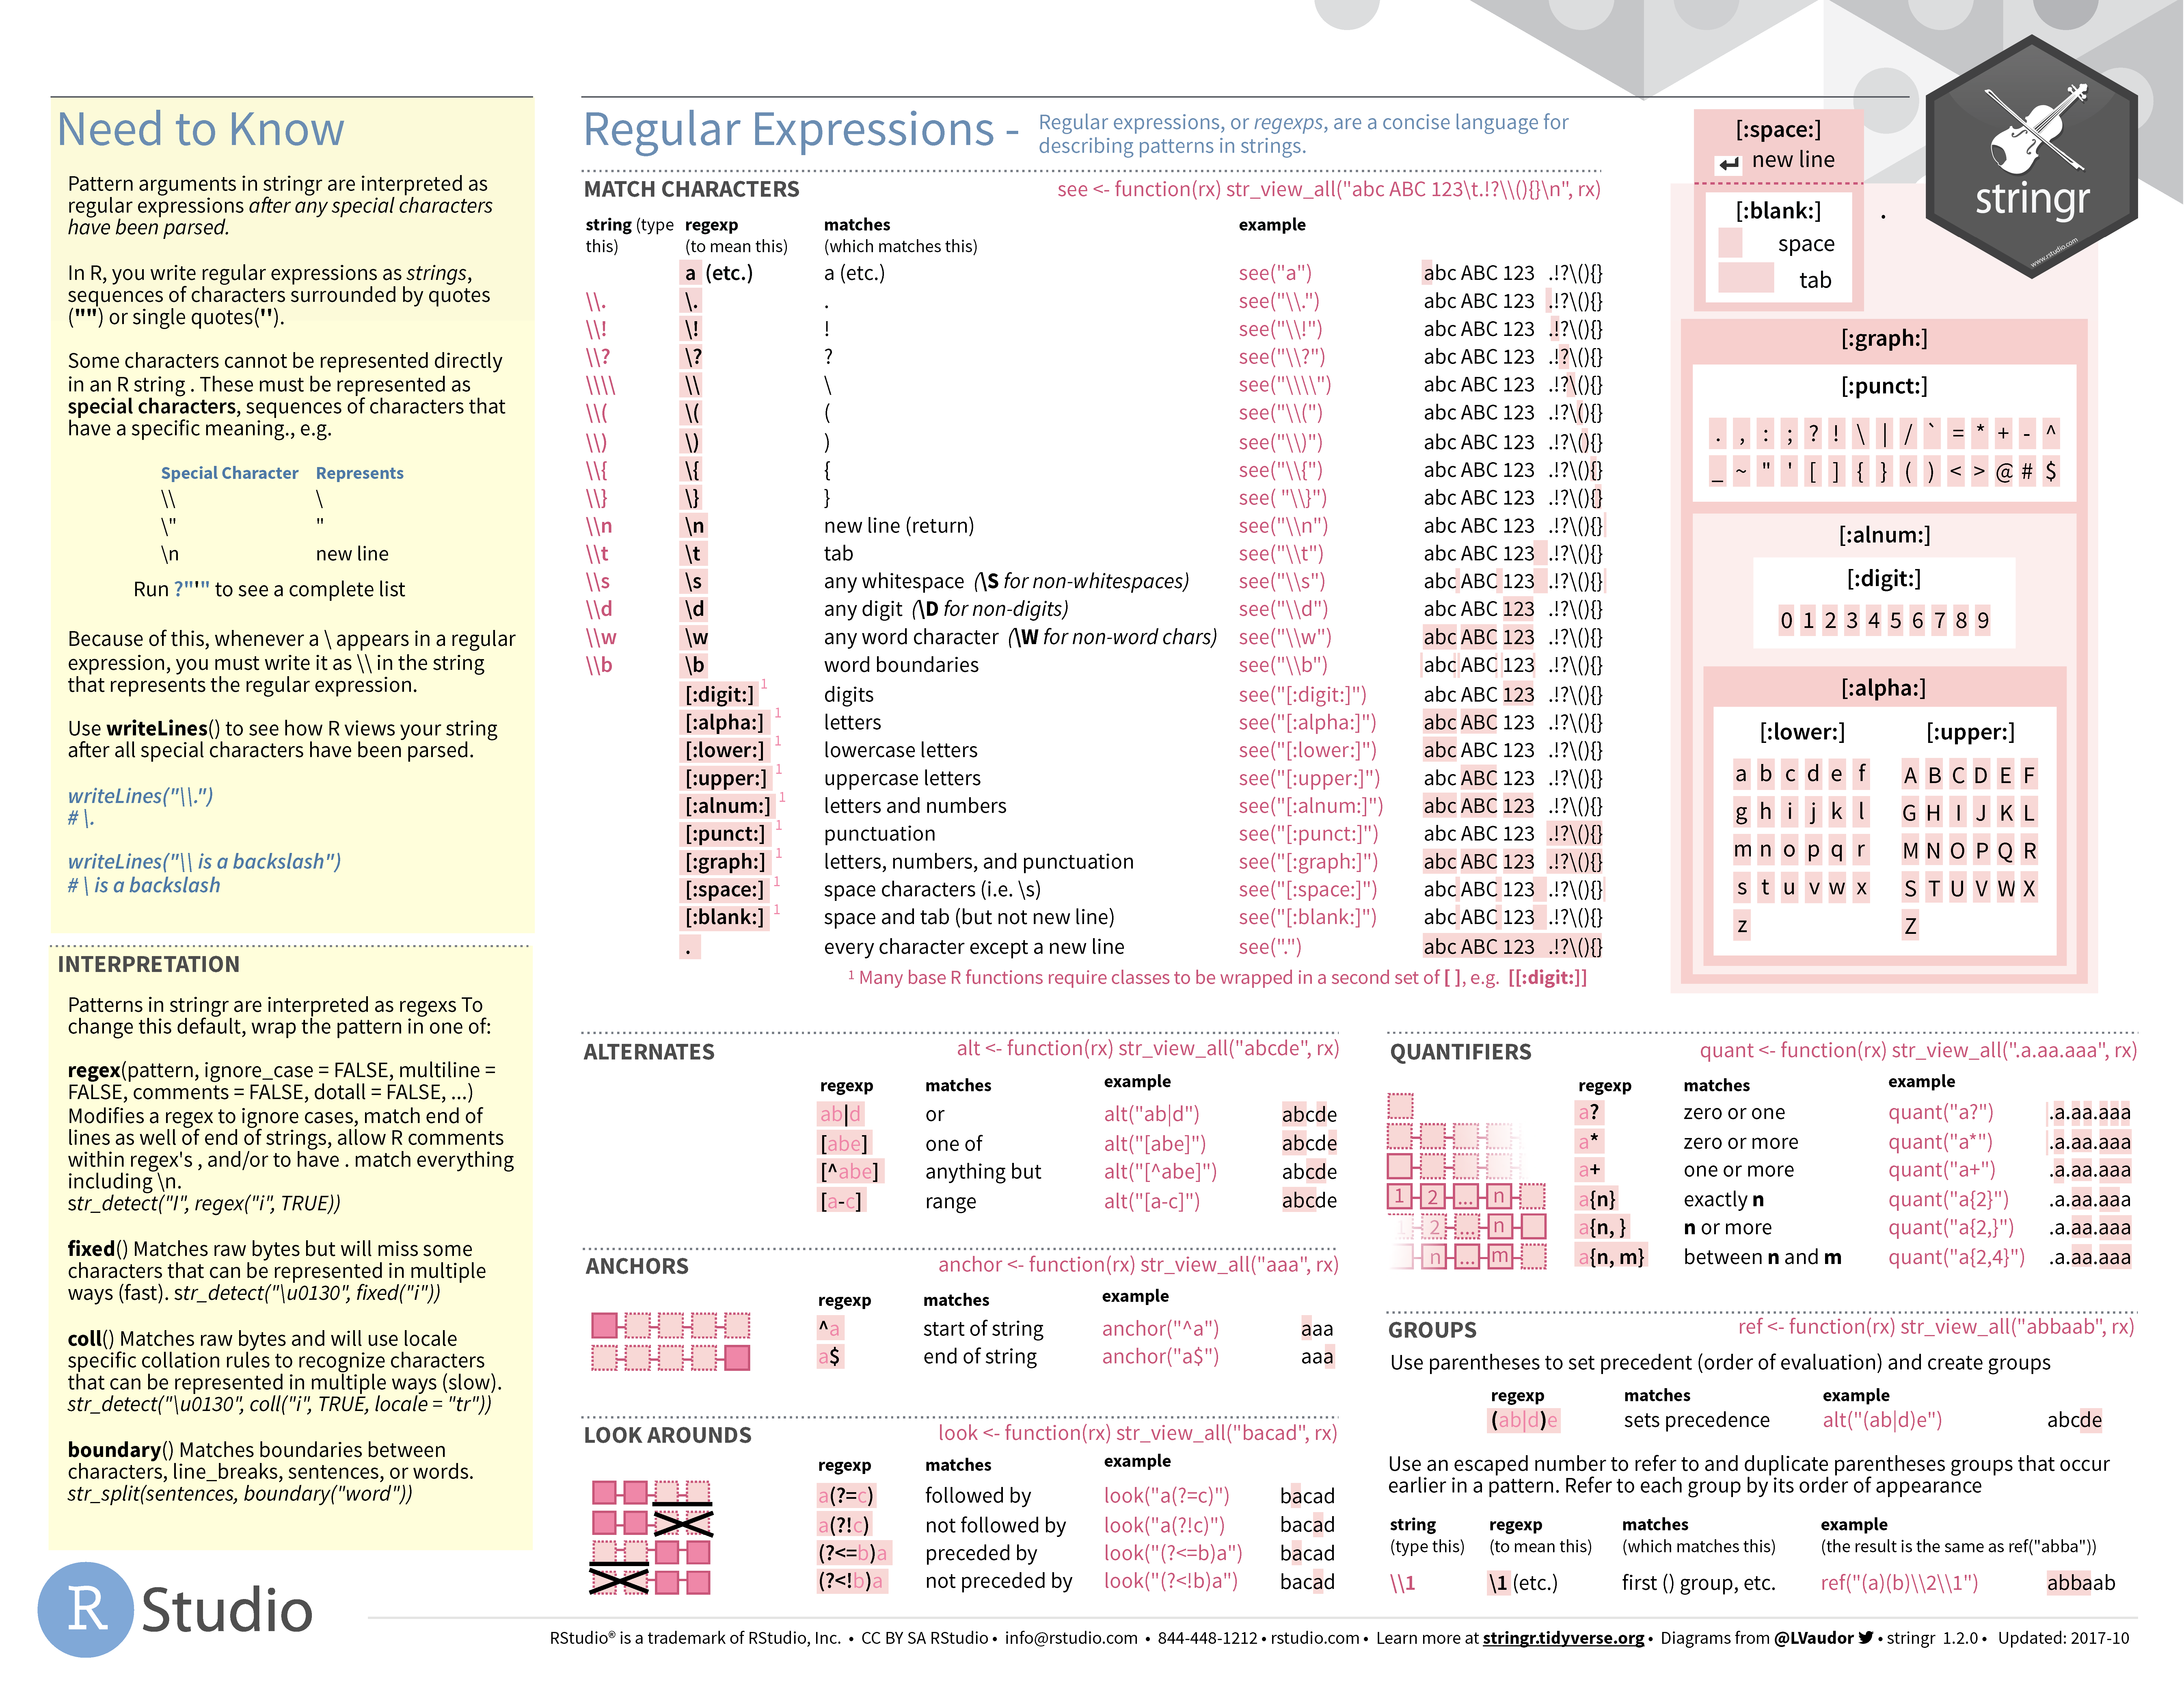
\includegraphics{images/regex.png}}}{Crédit: https://evoldyn.gitlab.io/evomics-2018/ref-sheets/R\_strings.pdf}}\label{cruxe9dit-httpsevoldyn.gitlab.ioevomics-2018ref-sheetsr_strings.pdf}}

\hypertarget{duxe9fi}{%
\subsection{Défi}\label{duxe9fi}}

\begin{enumerate}
\def\labelenumi{\arabic{enumi}.}
\tightlist
\item
  À partir de la table \texttt{rc}, composez un sous-ensemble de données
  comprenant seulement les longs-métrages produits par la
  Grande-Bretagne (GB).
\item
  Éliminez de ce sous-ensemble toutes les colonnes à l'exception de
  \texttt{TITRE\_ORIGINAL}, \texttt{TITRE\_FRANÇAIS}, \texttt{PAYS\_1.}
\item
  Quelle(s) fonctions pourrai(en)t vous renvoyer les dimensions de ce
  tableau de données? Exécutez-là et trouvez le nombre de lignes et de
  colonnes de ce sous-ensemble.
\item
  Combien de films de ce sous-ensemble contiennent, dans
  \texttt{TITRE\_FRANÇAIS}, le mot ``homme'' dans toutes ses
  déclinaisons (``Homme'' et ``homme'' au singulier et au pluriel)?
\end{enumerate}



\end{document}
